\section{PicoBlaze VHDL-Framework}
Die PicoBlaze Hardware-Platform bietet dem Benutzer eine begrenzte Anzahl von Bedienungselementen an, um gezielt mit den programmierten PicoBlaze-Applikationen interagieren zu k"onnen.
\begin{itemize}
	\item 8 LEDs, 8 Switches, 4-stellige 7-Segment-Anzeige
	\item Interrupt- und RESET-Button
	\item Auswahl der LogicPort-Signale
	\item LCD zur Anzeige von PicoBlaze Grundinformationen
	\item Bedientasten zur Kontrolle des Programmablaufs in Hardware
\end{itemize}

\subsection{Blockschaltbild}
\begin{minipage}{9cm}
	Neben den einfachen Bedienungselementen ist ein Interrupt-Controller integriert, der "uber die Signale \textbf{interrupt} und \textbf{interrupt\_ack} mit dem PicoBlaze verbunden ist.

	Die verf"ugbaren Peripherie-Komponenten lassen sich aus dem PicoBlaze Programm "uber die entsprechenden Input- bzw. Output-Ports ansprechen. Die Port-Adressen der verf"ugbaren Register sind wie folgt festgelegt:\\
	
		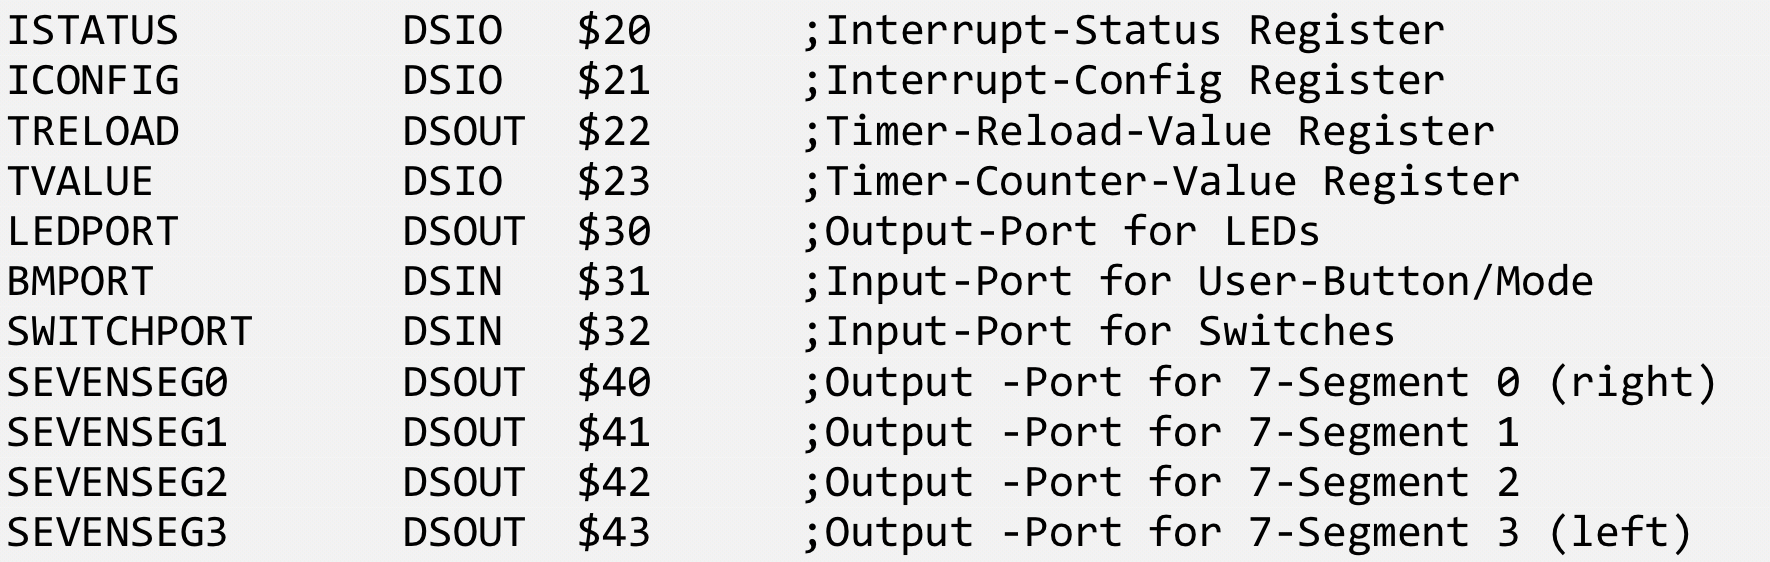
\includegraphics[width=9cm]{pics/8-Registeradressen}
		
	Die Beschreibung der Register kann im Quick-Reference gefunden werden.

\end{minipage}
%
\begin{minipage}{0.5cm}
	\ \
\end{minipage}
%
\begin{minipage}{9cm}
	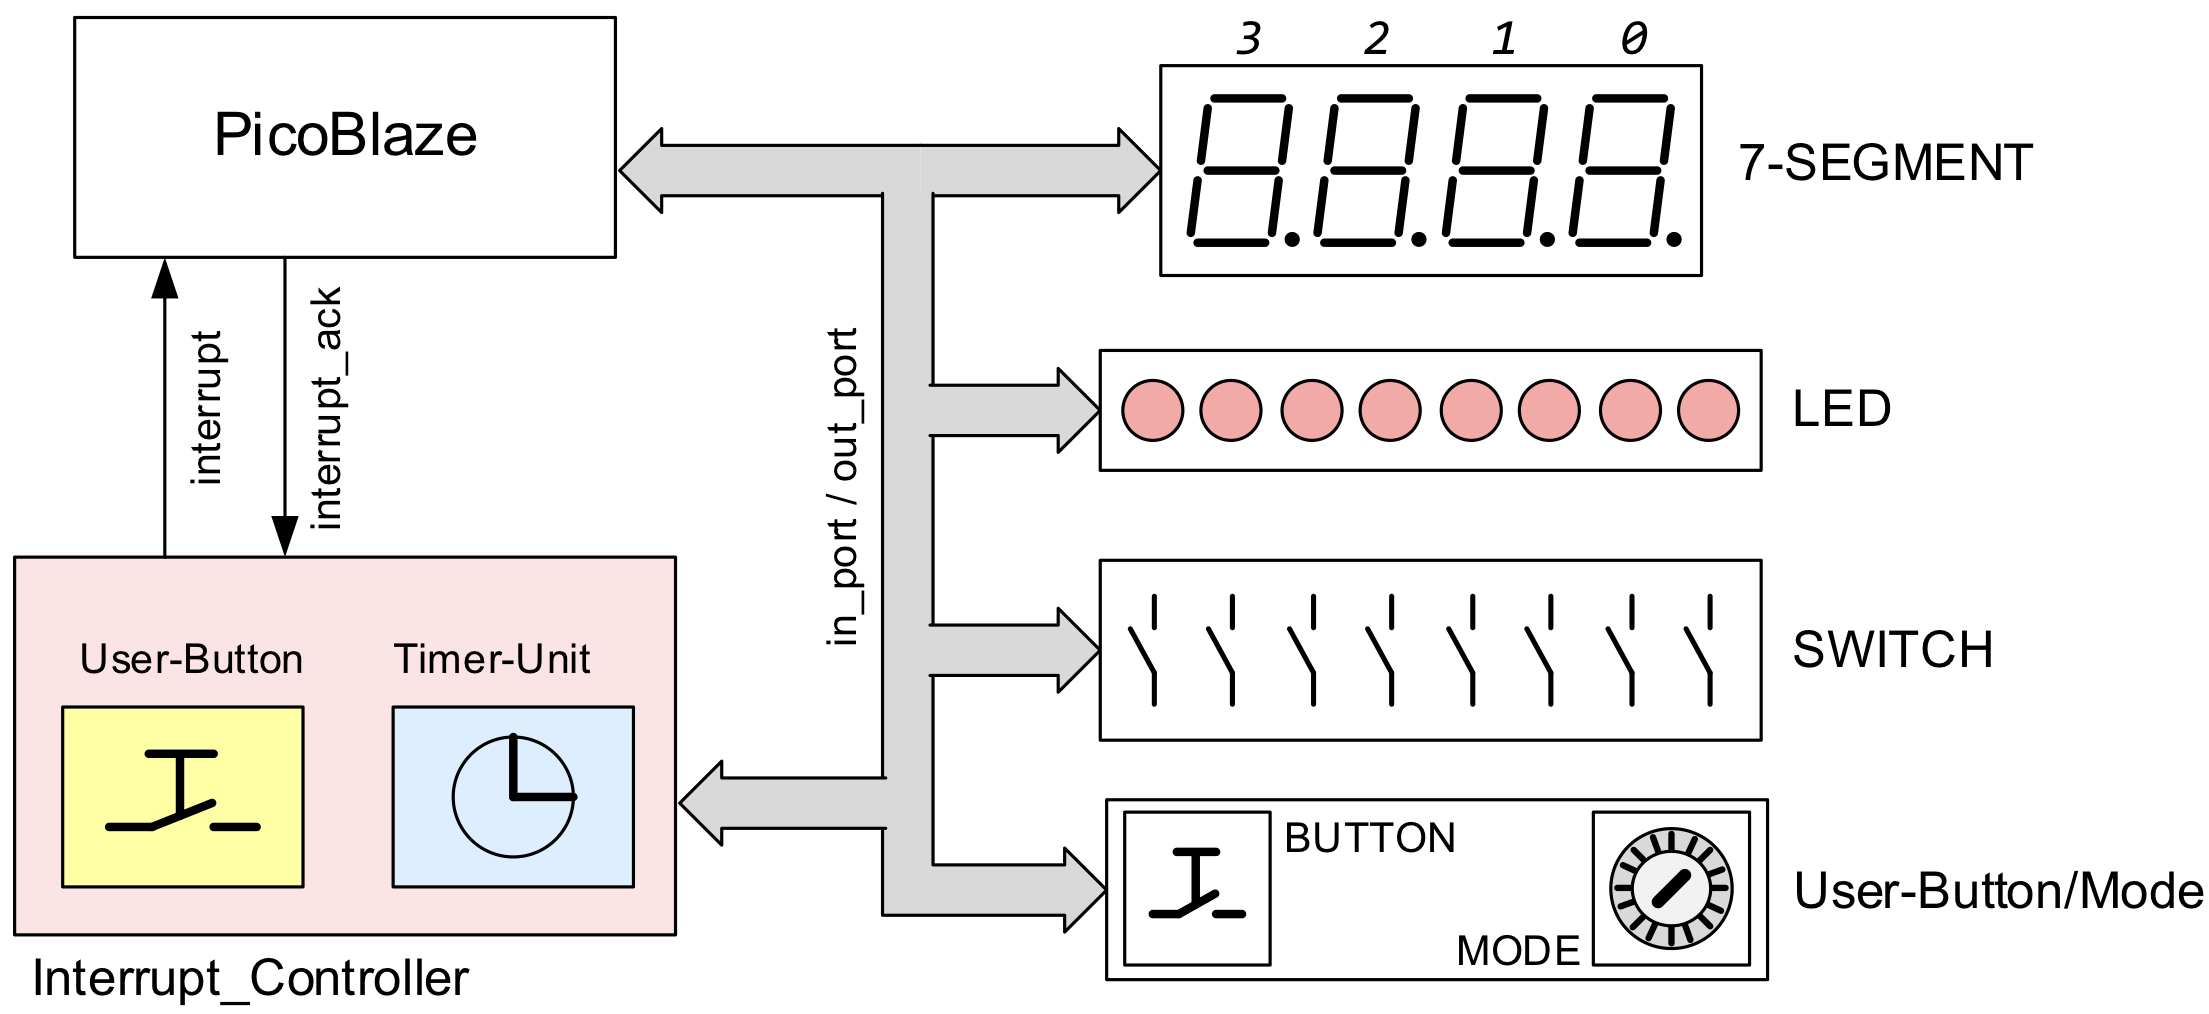
\includegraphics[width=9cm]{pics/8-Blockschaltbild}
\end{minipage}


\subsection{Interrupt-Controller}
Der PicoBlaze Softcore-Prozessor kann nur auf einen einzigen Interrupt von der umgebenen Peripherie reagieren und diese direkt verarbeiten.
Daf"ur ist auf der Hardware-Platform ein Interrupt-Controller in VHDL implementiert. Damit lassen sich Ereignisse von verschiedenen Interrupt-Quellen an den PicoBlaze signalisieren. Die verf"ugbaren Interrupts werden entweder manuell "uber den \textit{User-Button} oder automatisch "uber die integrierte \textit{Timer-Unit} ausgel"ost.

Zur Konfiguration und Steuerung der jeweiligen Interrupt-Quellen werden unterschiedliche Register ben"otigt:\\

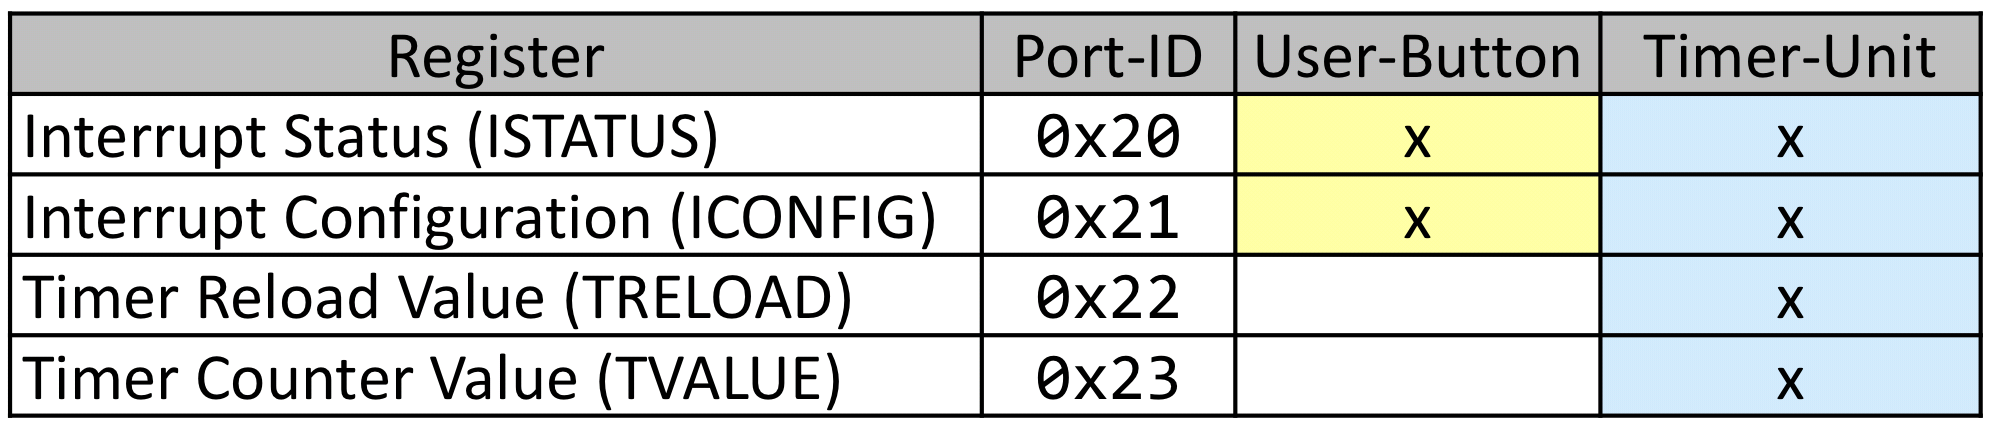
\includegraphics[width=9cm]{pics/8-Reg_InterruptController}

Damit keine \textbf{Race-Condition} entsteht m"ussen die Interrupt-Flags \textbf{BFLAG} und \textbf{TFLAG} aktiv auf 1 gesetzt werden um sie zu l"oschen. Wenn dies nicht so gemacht wird, w"urde eine "Anderung des Registers w"ahrend  Maskierung und Beschreiben nicht erkannt werden.

\subsubsection{Timer-Unit Interrupt}
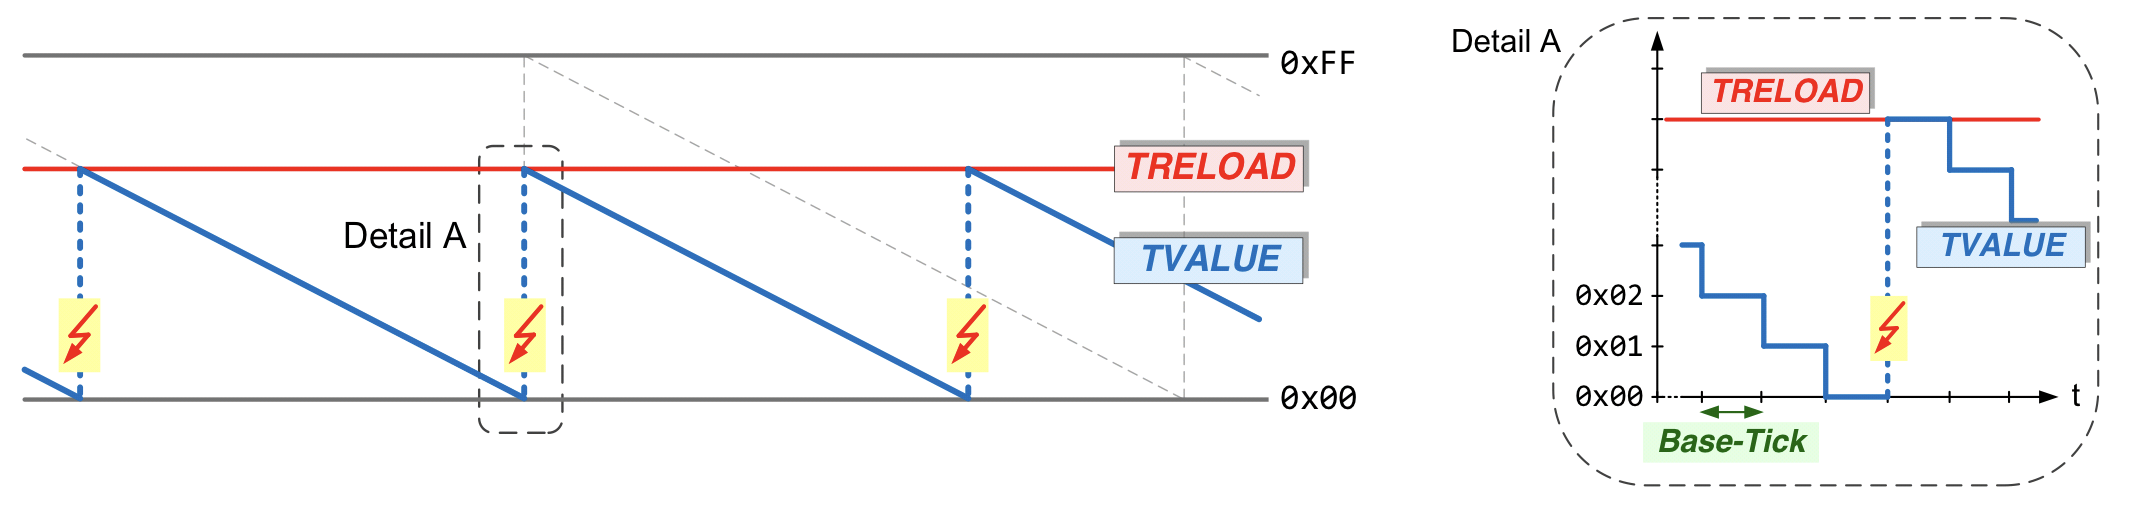
\includegraphics[width=15cm]{pics/8-TimingBlock}

Die Timer-Unit z"ahlt jeweils vom \textbf{TRELOAD}-Wert auf 0, somit wird jeweils nach folgender Zeit ein Interrupt ausgel"ost: (TRELOAD + 1) $\cdot$ Base-Tick

Die L"ange eines Base-Ticks kann im \textbf{ICONFIG-Register} unter \textbf{TBASE} eingestellt werden.

\subsubsection{Typischer Ablauf eines Timer-Unit Interrupt}
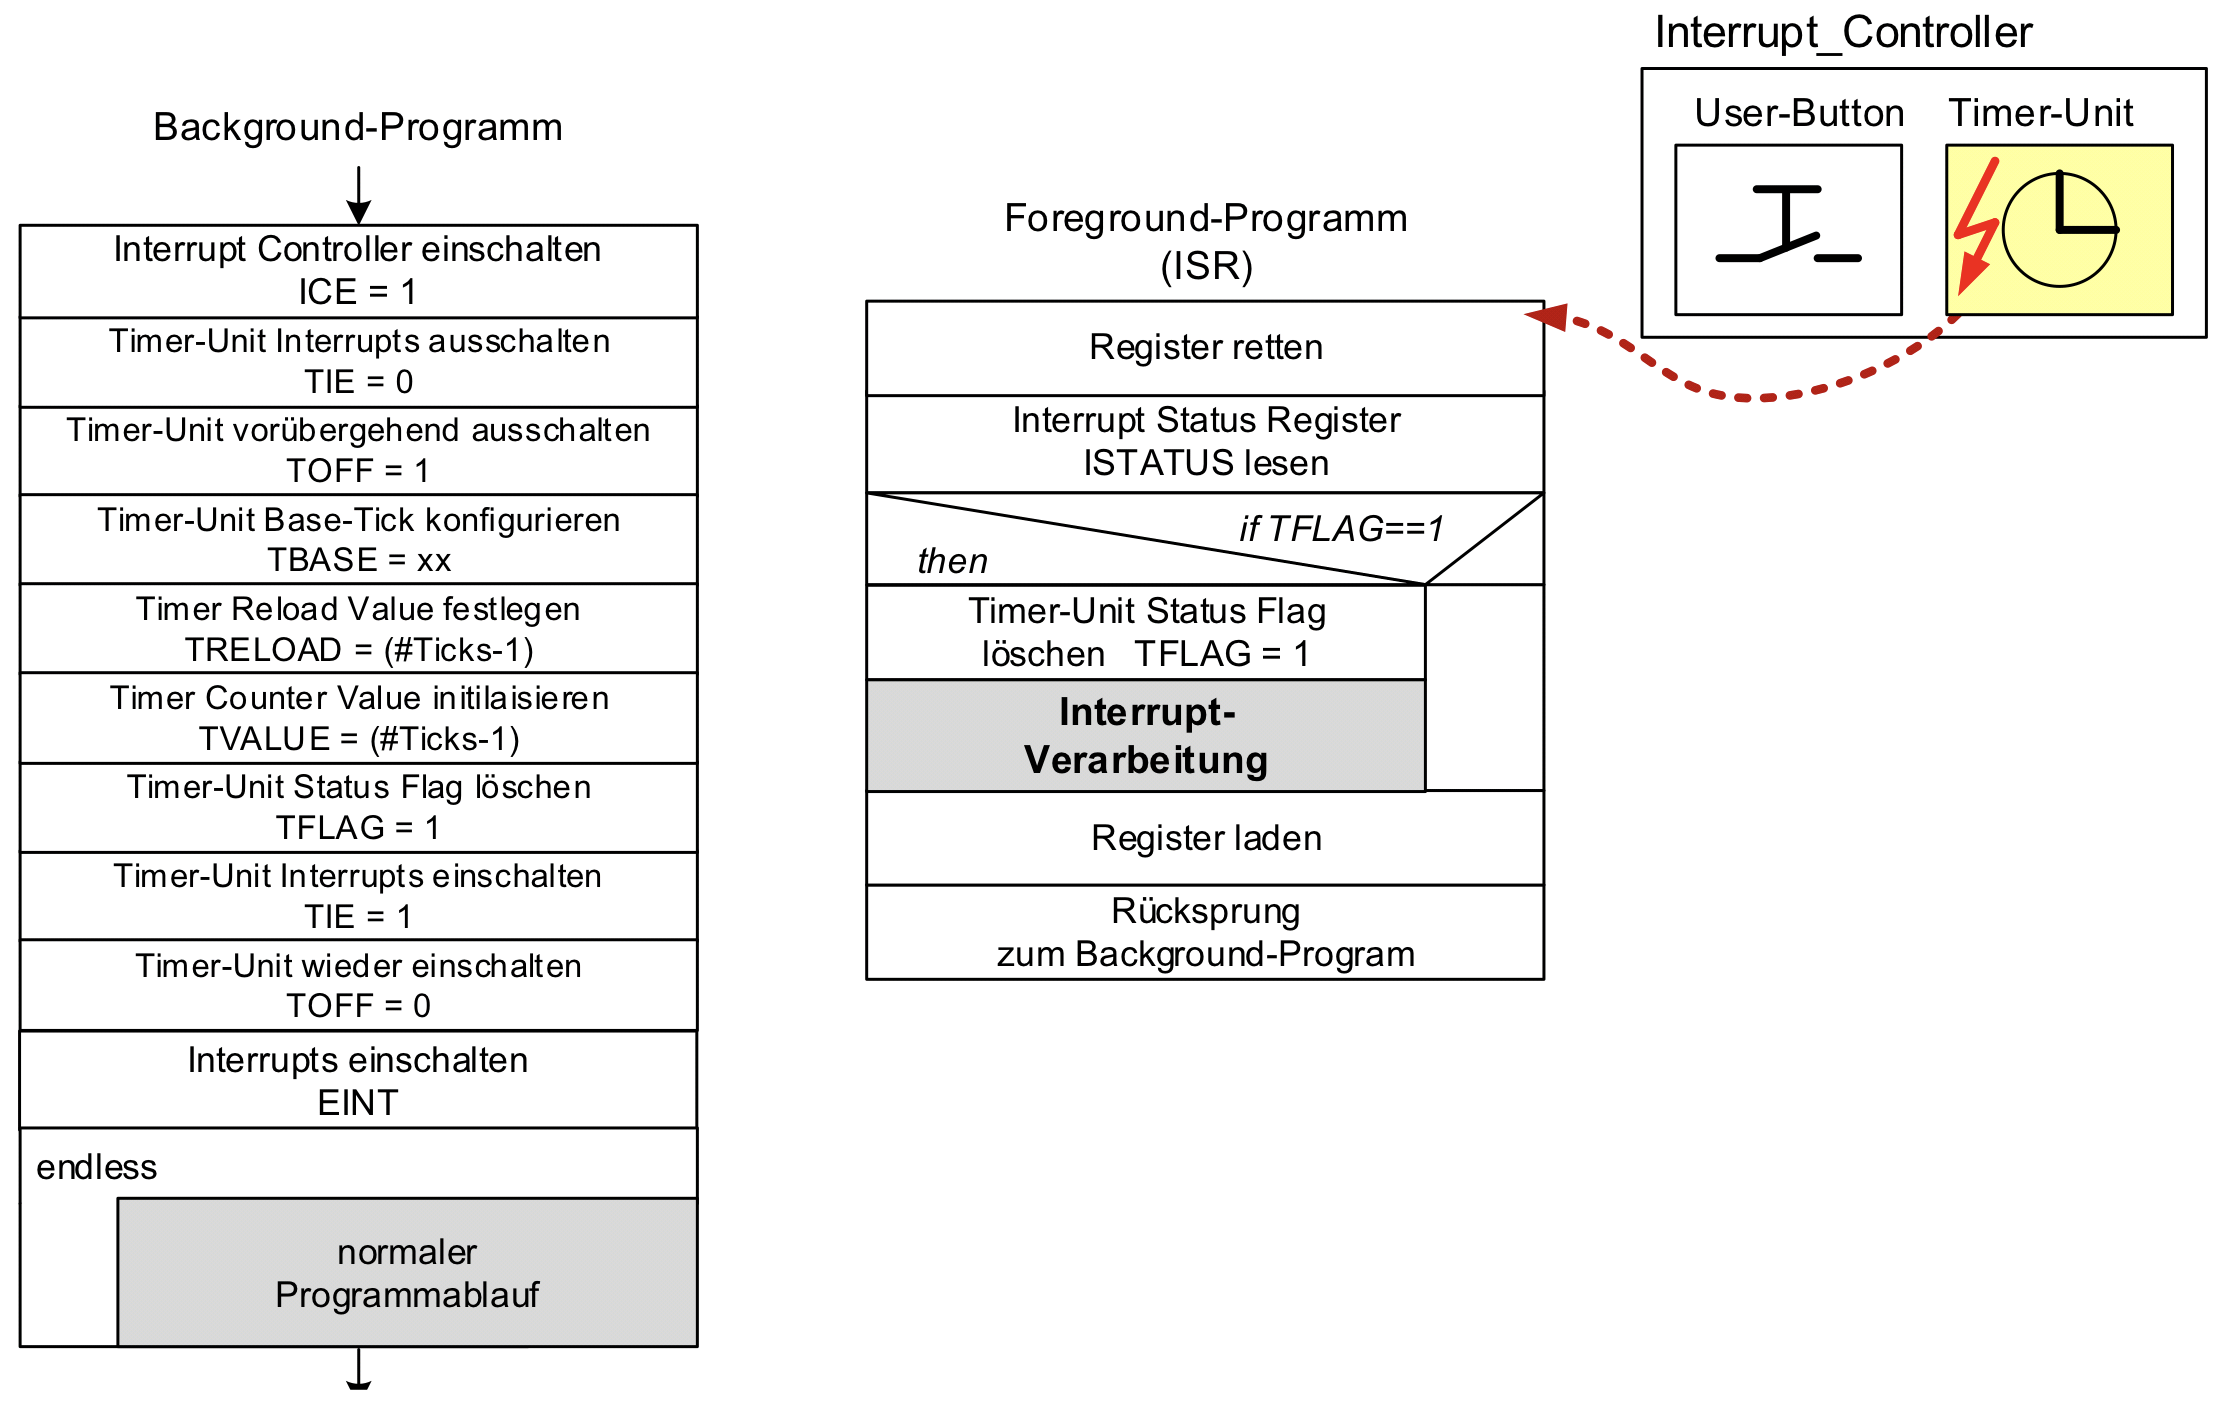
\includegraphics[width=18cm]{pics/8-Interruptablauf}

\subsubsection{Typischer Ablauf bei einem User-Button Interrupt}
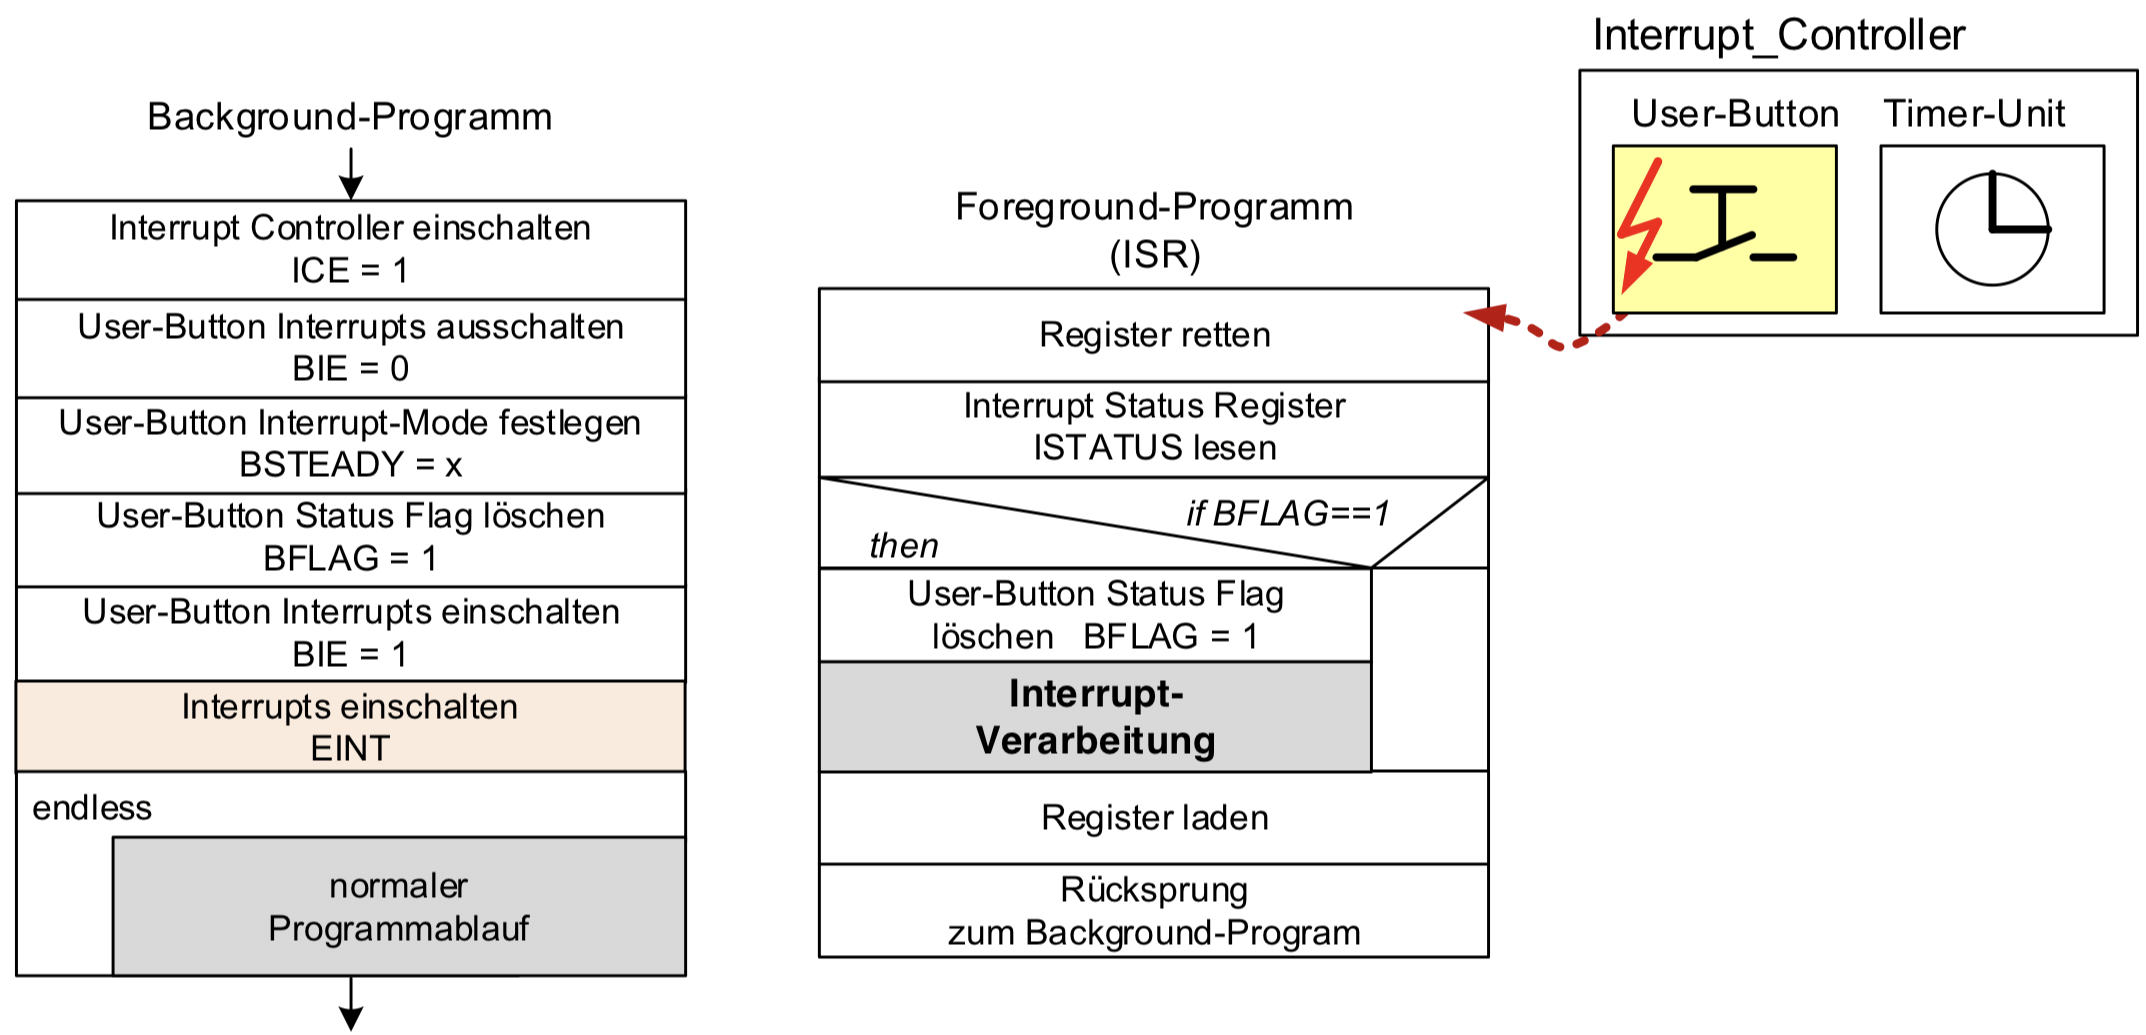
\includegraphics[width=18cm]{pics/8-User_Button_Interrupt}